%%                      COGSCI92.TEX
%% February 1992
%% Paper submitted to the Cognitive Science Conference, Indiana, 1992
%% Accepted April 1992
%% Requires the following files:
%%  ./              bib.bib
%%  ../postscript/  xrt.ps    xact.ps     xnet.ps     p3x8.ps
%%  ../inputs/errpc29.tex
%% COGSCI92.STY in $TEXINPUTS
%% psfig version 1.9
%% theapa version 2.5
%%%%%%%%%%%%%%%%%%%%%%%%%%%%%%%%%%%%%%%%%%%%%%%%%%%%%%%%%%%%%%%%%%%%%%%%%%
\documentstyle[COGSCI92,theapa,dectab,psfig]{article}
\begin{document}
\bibliographystyle{theapa}

\def\refname{References}
\citepunct{[}{\&}{\&}{ }{; }{, }{]}{}{.}
\citelabels{, ed.}{, eds.}{Vol.}{No.}{edition}%
{p.}{pp.}{chapter}{Technical report}

\psfigurepath{../postscript/}

% for multiplication \x34 produces 3x4 (only with a times sign)
\newcommand{\x}[2]{\mbox{$#1\times#2$}}
\newcommand{\X}[1]{\mbox{$#1\times$}}

\author{Richard Dallaway%
\thanks{Thanks to Harry Barrow \& David Young. Funded by the SERC in
conjunction with Integral Solutions Ltd. Simulations were performed using a
modified version of the \protect\citeA{pdp3} {\em bp} program, and POPLOG
POP-11.}
}
\email{richardd@cogs.susx.ac.uk}

\showwherepublished
\firstpage{558}

\title{Memory for Multiplication Facts}
\maketitle


\begin{abstract}
It takes approximately one second for an adult to respond to the problem
``\x78''. The results of that second are well documented, and
there are a number of competing theories attempting to explain the
phenomena \cite{camp85,ashcchil,siegmult}.
However, there are few fully articulated models available to
test specific assumption \cite{mcclmode}. This paper presents a
connectionist account of mental multiplication which models adult reaction
time and error patterns. The phenomenon is viewed as spreading activation
between stimulus digits and target products, and is implemented by a
multilayered network augmented with a version of the ``cascade''
equations \cite{mccascade}.  Simulations are performed to mimic Campbell \&
Graham's~\citeyear{camp85} experiments measuring adults' memory for
single-digit multiplication. A surprisingly small number assumptions
are needed to
replicate the results found in the psychological literature---fewer than
some (less explicit) theories presuppose.
\end{abstract}

\section*{Phenomena}

When asked to recall answers to two digit multiplication problems ``as
quickly and accurately as possible'' \cite{camp85}, both children and
adults exhibit well documented patterns of behaviour. In general, response
times (RTs) increase across the multiplication tables: problems in the nine
times table tend to take longer to answer than problems in the two times
table. However, this ``problem size effect'' has plenty of exceptions
(e.g., the five times table is much faster than its position would
suggest---see figure~\ref{rtplot}).  In addition, ``tie'' problems (\x22,
\x33 etc.)\ are recalled relatively quickly.
\citeA{camp85} found that adults under mild time pressure make errors at
the rate of 7.65 per cent, and 92.6 per cent of those errors fall into the
following five categories (after \citeA{mcclmode}):
%%
\begin{itemize}
%%
\item Operand errors, for which the erroneous product is correct for a
problem that shares a digit (operand) with the presented problem
(e.g., $\x64=36$, because the problem shares 4 with $\x94=36$).
%%
\item Close operand errors, a subclass of operand errors, where the
erroneous product is also close in magnitude to the correct product. That
is, for the problem \x{a}{b}, the error will often be correct for the
problem ($a\pm2) \times b$ or $a \times (b\pm2)$ (e.g., $\x64=28$).  This
phenomenon is referred to as the ``operand distance effect''.
%%
\item Frequent product errors, where the error is
one of the five products 12, 16, 18, 24 or 36.
%%
\item Table errors, where the erroneous product is the correct answer to
some problem in the range \x22 to \x99,
but the problem does not share any digits with the presented
problem (e.g., \x64=15).
%%
\item Operation errors, where the error to \x a b is correct for $a+b$.
\end{itemize}

\begin{figure}[tbh]\centerline{\fbox{\vbox{%\vspace{1mm}%
\psfig{file=xrt.ps,width=\columnwidth}%\vspace{1mm}%
\caption{Plot of mean correct RT per multiplication table collapsed over
operand order for mean RT of: 60 adults \protect\cite[app.~A]{camp85}; 26
children in grade 5, RT scaled down from a range of 1.19--2.97 seconds to
fit graph [ibid. app.~B]; 20 networks trained on skewed frequencies; and,
the same 20 networks after continued training on uniform frequencies. The
RT for both networks has been scaled by the same amount.}
\label{rtplot}}}}\end{figure}

Despite being drilled on the multiplication tables at school, children and
adults make these systematic slips in recall. The problem is to produce a
model which has correctly learnt the multiplication tables, yet can make
slips when recalling answers. Given the observations on the types of
erroneous responses, and the RT for correct responses, what assumptions
must be made to account for these phenomena? The model presented here
suggests that the initial skew in the frequency and order of presentation
of multiplication facts \cite[p.~118]{camprole} is one of the important
factors.

%%%%%%%%%%%%%%%%%%%%%%%%%%%%%%%%%%%%%%%%%%%%%%%%%%%%%%%%%%%%%%%%%%%%%%%%%%%
\section*{Architecture of the model}



The structure of the network is shown in figure~\ref{xnet}.  This
architecture has evolved in a number of stages since it was first used as a
subnetwork in a sequential network for long addition (and later long
multiplication).  Initially the output layer was divided into ``tens'' and
``units'', and by adding a simple RT measure it was found that the network
produced a prominent dip in the RT curve for the five times table.  This
effect was increased by training sequentially through the tables, but the
network did not produce the kinds of mistakes reported by \citeA{camp85}.
Changing the output layer to a representation of products, and using a
coarse encoding of the input digits produced more realistic errors.


The current network is trained on all the problems \x22 through \x99 in a
random order using backpropagation. %(learning rate 0.01, momentum 0.9).
%
The two digits that comprise a problem are coarse encoded on the two sets
of eight input units, with the activation decaying exponentially from the
presented digit (e.g., when encoding ``5'', the input vector would contain
1.0 for the five unit, and 0.5 for the four and six units, and so on). For
tie problems, an additional tie bit is set to 1.0. Without this, the tie
problems were consistently among the slowest problems. The tie bit can be
thought of as reflecting the perceptual distinctiveness of tie problems.
Activation flows through a hidden layer of ten units to the output layer.
There is one output unit per product type plus a ``don't know'' unit.  The
network is trained to activate one output unit per problem (a one-of-N
encoding).

During training the presentation frequency of each pattern is linearly
skewed in favour of the smaller problems (relative frequency of 1.0 for
\x22 to 0.1 for \x99, based on correct product). Although small problems do
occur more frequently in textbooks, there is no reason to believe this skew
continues into adulthood \cite[p. 328]{mcclmode}.  Hence, after training to
an error criterion (total sum squared, TSS) of 0.05 on the skewed training
set (taking approximately 8~000 epochs), the network is trained for a
further 20~000 epochs with equal frequencies (reaching a mean TSS of
0.005).  At the end of training both the ``skewed'' networks and
``equalized'' networks correctly solve all problems. An initial worry was
that the skew would lead the networks into a local
minima from which the task could not be completed. To avoid this
possibility, a low learning rate of 0.01 was used during training (momentum
was 0.9).

The skew was produced by storing the relative frequency (between zero and
one) of a problem alongside the problem in the training set.  When a
problem was presented to the network, the weight error derivative was
multiplied by the relative frequency value for that pattern. (This can be
thought of as providing each input pattern with a different
learning rate.) This method allowed accurate control over the presentation
frequencies, without duplicating entries in the training set.


The ``cascade'' activation equation
\cite[p.~153]{pdp3} is used to simulate the
spread of activation in the network. Each unit's activation is allowed
to build up over time:

\def\net{\mbox{net}}
$$ \net_i(t) = k \sum\limits_j w_{ij} a_j(t) + (1-k)\ \net_i(t-1), $$


\noindent where
$k$ is the cascade rate which determines the rate with which activation
builds up, $w$ is the weight matrix, and $a_j(t)$ is the activation of unit
$j$ at time $t$. For the simulations described here, $k=0.05$. The $\net_i$
is passed through a logistic squashing function to produce the activation
value, $a_i$.  The response values are taken to be the normalized
activation values (the sum of the output layer activity is 1.0).

\citeA{pdp3} point out that the asymptotic activation of units under the
cascade equation is the same as that reached after a standard feed-forward
pass.
Hence, the network is trained without the cascade equation (or with
$k=1$, if you prefer), and then the equation is switched on to monitor
the network's behaviour during recall.

At the start of cascade processing the initial state of the network is the
state that results from processing an all-zeros input pattern. This gives a
common starting point for all problems.
The network
is trained to activate the ``don't know'' unit  for an all-zeros input.
Figure~\ref{actplot} is a time plot of output activation using
the cascade equations.


%%%%%%%%%%%%%%%%%%%%%%%%%%%%%%%%%%%%%%%%%%%%%%%%%%%%%%%%%%%%%%%%%%%%%%%%%%%
\section*{Simulations}

\subsection*{Method}

On each trial (presentation of a problem) the network
randomly selects a threshold between 0.4 and 0.9.  Processing then starts
from the all-zeros (``don't know'') state, and proceeds until a product
unit exceeds the threshold. The RT (number of cascade steps) is recorded
for a correct response, and erroneous responses are classified into the
five categories itemized above. The network is presented with each of the
64 problems 50 times, and the mean correct RT is recorded.  This is
repeated with 20 different networks (different initial random weights).

Given enough time (usually no more than 50 cascade steps), the network
will produce the correct response for all 64 problems. For example,
figure~\ref{actplot} shows the response of a network to the problem \x38.
After the ``don't know'' unit has decayed, the unit representing 27 becomes
active until the network settles into the correct state, 24.  This is a
demonstration of the operand distance effect, but there is slight
activation of other products: $\x37=21$, $\x28=16$, $\x48=32$, $\x33=9$,
and $\x27=14$.

With a high threshold the networks will
reliably produce the correct response to a problem. However, early in
processing erroneous products are active (e.g., 27 in
figure~\ref{actplot}),
and with a low threshold these
errors are reported. Note that this is rather different to previous
connectionist (Brain-state-in-a-box, BSB) model of mental arithmetic
\cite{viscmemo,andestud}.
The full details of the BSB model have not yet been
published, and only small scale simulations have been performed.  In
essence, the model is an auto-associator that settles into attractor states
representing the answer to the presented problem.  However, this means that
the model, as presented, simply lacks the ability to correctly answer some
problems, or fails to respond at all.  This runs against the notion that
slips are one-off run-time errors, rather than permanent disabilities.
\citeA{mcclmode} comment that the \citeA{viscrepr} ``proposal has several
limitations and cannot be considered a well-articulated model'', but add
that ``the [neural net] approach probably merits further exploration''
[p.~395].

\begin{figure}[bth]\centerline{\fbox{\vbox{\vspace{2mm}%
\psfig{file=xnet.ps,width=\columnwidth,height=3.5cm,angle=0}
\caption{}\label{xnet}}}}\end{figure}

\begin{table*}
\fbox{\vbox{\vspace{2mm}
\begin{center}

\def\noteast{\hspace{-1.5em}\mbox{\raise 1mm\hbox{\footnotesize$\ast$}}}
\def\notedag{\hspace{-1.5em}\mbox{\raise 1mm\hbox{\footnotesize\dag}}}
\setdec 00.0

\begin{tabular}{lcccl}
&\multicolumn{2}{c}{Networks}&Adults&\\
&Skewed&Equalized&&\\
Operand errors          &\dec 90.04 &\dec 86.51 &\dec 79.1 &\\
Close operand errors    &\dec 78.98 &\dec 73.75 &\dec 76.8 &\noteast\\
Frequent product errors\notedag &\dec 27.76 &\dec 23.68 &\dec 30.6 &\\
Table errors            &\dec 9.74  &\dec 13.49 &\dec 13.5 &\\
Operation error         &\dec 3.98  &\dec 3.22  &\dec 1.7 &\noteast\\
Error frequency         &\dec 14.10 &\dec 18.64 &\dec 7.65 &\smallskip\\
\multicolumn{5}{c}{\footnotesize$\ast$ Approximate percentage.}\\
\multicolumn{5}{c}{\footnotesize\dag Percentage of operand errors.}
\end{tabular}

\end{center}
\caption{Percentage breakdown of errors. Figures are mean values from
twenty different networks, and mean values from sixty adult subjects
\protect\cite[app.~A]{camp85}.  Note that the model has not been
trained on addition facts, so the frequency of operation errors is
coincidental.}
\label{errorpc}
}}\end{table*}


\begin{figure}\centerline{\fbox{\vbox{
\psfig{file=p3x8.ps,width=\columnwidth,height=7cm}
\caption{Response of the output units over 40 time steps for the problem
\x38.  Output units representing products over 32 are not shown on this
graph.}\label{actplot}}}}\end{figure}

\begin{figure}\centerline{\fbox{\vbox{%\vspace{1mm}%
\psfig{file=xact.ps,width=\columnwidth}%[65]\vspace{3cm}
\caption{Hidden unit activation for one network.
Each large rectangle represents one
hidden unit.  Within each rectangle, the size of the smaller rectangles
represents
the activation of the hidden unit to a particular problem. Each large
square mimics the multiplication table (top-left for \x22,
and bottom-right for \x99). For example,
unit~22 responds to problems in the three and four times tables.
}\label{xact}}}}\end{figure}

\subsection*{Results}

The mean RTs plotted in figure~\ref{rtplot} show some
of the basic features of the problem size effect.  For the skewed networks
the RT correlates $r=0.36$ ($p=0.0018$) with adult RT \cite{camp85}. This
falls to $r=0.19$ ($p=0.063$) after substantial training on the equalized
patterns.  Note that the RTs have reduced and flattened out for the
equalized network, which is just what is expected after continued practice
\cite[p.~349]{camp85}. The obvious feature of the RT plot is the drop in RT
for the nine times table.  Children in grades 3 to~5 respond faster to \X9
than \X8 problems \cite{camp85}, but this levels out for adults.

The inclusion of a ties unit is necessary to ensure that ties are among the
fastest problems.  Implicit in this is an assumption that there is
something perceptual about ties which results in a flagged
encoding---perhaps the effect of being taught the notion of ``same'' and
``different''. The RTs
of 6 (out of 8) of the tie problems were below the mean RT for their
table, increasing to 7 ties for the equalized networks (\x66 remaining
above the mean for the six times table).

Table~\ref{errorpc} shows the error
percentages of the networks compared to those of adults.  Both sets of
networks have error distributions that are similar to that of adults, and
there is little difference between the skewed and equalized
networks.

It should be noted that human subjects sometimes respond with a number that
is not a correct product for any of the problems \x22 to \x99 (e.g.,
$\x23=5$). The current network cannot produce non-table errors. However,
\citeA{camp85} report that only 7.4 per cent of errors are of this kind.
(An account of non-table errors might begin by augmenting the network with
a tens and units read-out layer.)

A further point of interest is the correlation between problem error rate
and correct RT. \citeA[p.~110]{camprole} reports a correlation of 0.93 for
adults.  For the skewed and equalized networks $r=0.74$
and $r=0.76$ respectively.  It is not obvious that any model
would necessarily predict that slower problems produce more errors.




\subsection*{Analysis}

RT depends on
the net input to a unit, and this can be increased by having some large (or
many small) weights.  Although there is no easy way to determine why
certain weights develop, some of the factors involved can be
described.

The presentation frequency of a problem and product should have a strong
effect on the weights: those problems seen more often should develop
larger weights. Simulations with networks trained only on patterns with
equal presentation frequencies have demonstrated that the frequency of
presentation is important. Typically these networks produce
high-frequency products as errors, and have poor correlations to human RT.

Frequency does not explain why the five times table should be faster than
the four times table. ``Product uniqueness'' may explain why:
none of the products in the five times table occur outside the
context of five (unlike the two times table, where the products 12,
16 and 18 occur in other tables).  Hence, the error signals for the
fives products are not diluted through differing hidden
representation for different problems.  The same is true of the seven
times table, but for a lower presentation frequency.

The nine times table has the largest range of all the tables. This seems to
give the table a RT advantage because many hidden units respond
to the nine times table: the nine times table is the third ``most encoded''
problem (typically five hidden units respond to the nine times table; seven
for the two times tables; six to the three times). This is because the
hidden units respond to a range of input problems.  For example,
figure~\ref{xact} shows that unit~26 responds to small products; unit~23 to
medium products; and unit~24 responds to larger products. %%goldilocks%%



The hidden units' preference for responding to bands of inputs explains the
mechanism behind the operand distance effect. Hidden units' activities
change smoothly during the course of processing, but at differing rates.
This change affects groups of related products, and due to the overlap in
encoding (e.g., between unit~23 and 24 in figure~\ref{actplot}), some
hidden units may force incorrect products to exceed threshold.


\section*{Discussion}
Apart from the training frequency skew, the other main
assumption of the model is the coarse coding of the input pattern.  The
importance of this assumption has been demonstrated by simulations using a
one-of-N input encoding (the same encoding that was used for the outputs).
The results of those simulations produced comparable RT correlations, but
poor error distributions.  The assumption is that the coarse encoding is
due to general knowledge of number (perhaps from counting).

This study has focused on mean adult performance on the problems \x22
to \x99 because these problems have detailed published results. There are
persistent statements in the literature that zero and one times tables are
governed by procedural rules (e.g., \citeA[p.~341]{camp85};
\citeA[p.~51]{millcogn}; \citeA[p.~334]{staznetw}). The motivation for this
seems to stem from the fact that it is easy to produce answers for the zero
and one tables. Initial experiments with the architecture confirm what is
expected of backpropagation when the zero and one times tables are included
in the training set. The zero table is by far the fastest and least prone
to error, followed by the one times table.  This is consistent with RTs
reported by \citeA{millcogn}.  On this basis there is no reason to assume
that there is a separate mechanism for the zero and one tables.

Some of the assumptions posed by other models may be accounted for by
differences in methodology.  For example, in models that assume direct
links (no hidden units) between stimulus digits and target products there
must be additional information for the model to be capable of producing the
correct answer.  There must be either: different (token) answer nodes for
each problem (e.g., multiple copies of the ``12'' node for \x26 and \x34 as
used by \citeA{ashcchil}); or input nodes representing whole problems (e.g.
a ``\x34'' input node as in \citeA{camp85}); or both \cite{siegmult}.

However, other assumptions were not found to be needed in this model.  For
example, there was no need for explicitly learning incorrect associations,
as suggested by both \citeA{siegmult} and \citeA{camp85}.  Nor was there
need for connections between product units (\citeA{camp85} and
\citeA{ashcchil}), nor connections from general ``magnitude'' units as used
by \citeA{camp85}.   These models have been criticised by \citeA{mcclmode}
for not specifying the rationale for these additional connections.

Of course, there are a number of shortcomings to the model presented here.
There is no empirical evidence to suggest
that adults are exposed to a skew in the frequency of
multiplication problems, and this was modelled by further training the
skewed networks on equal frequency problems.  Although the RTs for the
equalized networks diverge from the adult RTs, they retain the basic
features of the problem size effect and error distributions.  One
conclusion that can be drawn from this is that it is quite possible for the
effect of training on skewed problems to continue to be felt even after a
significant period of training on non-skewed problems.

As it stands the model makes no attempt to account for a number of
important aspects of arithmetic. Future
directions for this work could focus on: modelling single digit addition;
the
role of back-up (counting) procedures; error priming; and the model's
position in long (multi-digit) arithmetic procedures.

The backpropagation cascade model presented here has detailed the spread of
activation, response selection, training regime and minimal assumptions
needed to replicate results on adult performance.  This has been done in
the context of attempting to mimic the experiments performed by
\citeA{camp85}, and hence the results are of a statistical nature.  The
explicitness of the model is one of its strong points, and as
\citeA{mcclmode} point out it is now time to ``shift from a
demonstration of the framework's basic merit to the hammering out of
detailed, fully elaborated models'' [p.~394].  This has been an attempt to
do just that.

\bibliography{bib}
\end{document}
